\subsection{Функция Грина уравнения Лапласа первой краевой задачи в круге, на полуплоскости в полупространстве. Метод отражений.}
%autor: Сеня, Слава (первый раздел)
\subsubsection{Введение. Основная формула Грина}
\paragraph{Случай $ \mathbb R^3 $.}
Ранее была получена \emph{вторая формула Грина} \eqref{eq:green2}. Легко
заметить\footnote{Надо записать уравнение Лапласа в сферических координатах, где
функцию $ v $ считать зависимой только от $ r $ и проинтегрировать ОДУ.}, что
функция $ v(M) = 1/R_{MM_0} $ является гармонической\footnote{То есть
  удовлетворяет уравнению Лаплама. Символом $ R_{MM_0} $ обозначается расстояние
$ MM_0 $.} при $ M \neq M_0 $. Подставим эту функцию во вторую формулу Грина для
некоторой области $ T\setminus U(M_0; \varepsilon) $\footnote{Обозначения: $ U(M_0;
\varepsilon) $ --- шар с центром в особой точке $ M_0 $ и радиусом $ \varepsilon
$; $ \partial U(M_0; \varepsilon) $ --- его граница.}, где нет особых точек: 
\[
  \iiint\limits_{T\setminus U} \left( u\Delta \frac{1}{R} - \frac{1}{R}\Delta u \right)
  dxdydz = \iint\limits_{\partial T} \left( u \frac{\partial}{\partial n}
  \left(\frac{1}{R}\right) - \frac{1}{R} \frac{\partial u}{\partial n} \right)
  \,d\sigma + \iint\limits_{\partial U} u \frac{\partial}{\partial n} \left(
  \frac{1}{R} \right) \, d\sigma - \iint\limits_{\partial U} \frac{1}{R}
  \frac{\partial u}{\partial n}\,d\sigma.
\]
Теперь заметим, что 
\begin{align*}
  \frac{\partial}{\partial n} \left( \frac{1}{R} \right) \bigg|_{\partial U} &= -
  \frac{\partial}{\partial r} \left( \frac{1}{R} \right) \bigg|_{r=\varepsilon} =
  \frac{1}{\varepsilon^2},\\
  \iint\limits_{\partial U} u \frac{\partial}{\partial n} \left( \frac{1}{R}
\right)\, d\sigma &= \frac{1}{\varepsilon^2} 4\pi\varepsilon^2 u^\ast = 4\pi
  u^\ast,
\end{align*}
где $ u^\ast $ --- среднее значение функции $ u(M)|_{\partial U} $. Аналогично 
\[
  \iint\limits_{\partial U} \frac{1}{R} \frac{\partial u}{\partial n}\,d\sigma =
  \frac{1}{\varepsilon} 4\pi\varepsilon^2 \left( \frac{\partial u}{\partial n}
  \right)^\ast = 4\pi\varepsilon \left( \frac{\partial u}{\partial n}
  \right)^\ast.
\]
Заметим также, что при $ \varepsilon \to 0 $ верно $ u^\ast \to u(M_0) $ и $
4\pi\varepsilon (\partial u/\partial n)^\ast \to 0 $. Так мы пришли к
\emph{основной интегральной формуле Грина} 
\begin{equation}\label{eq:green3}
  4\pi u(M_0) = - \iint\limits_{\partial T} \left[ u(P) \frac{\partial}{\partial
  n} \left( \frac{1}{R_{M_0 P}} \right)  - \frac{1}{R_{M_0 P}}\frac{\partial
u}{\partial n} \right] \,d\sigma - \iiint\limits_T \frac{\Delta
u(M)}{R_{M_0M}}\,dxdydz,
\end{equation}
где $ P $ --- некоторая граничная точка области $ T $. До этого предполагалось,
что $ M_0 \in T $. При $ M_0 \in \partial T$ несложно прийти к формуле
\eqref{eq:green3}, где слева вместо $ 4\pi $ стоит $ 2\pi $ (поскольку там имеем
вместо $ U(M_0; \varepsilon) $ поверхность, чей объём при малых $ \varepsilon $
близок к половине объёма шара). Если $ M_0 $ не
принадлежит замыканию $ T $, то функция $ v $ гармонична во всей области, и
вместо $ 4\pi $ следует поставить ноль.

\paragraph{Случай $ \mathbb R^2 $.}
Совершенно аналогично, только для гармоничности теперь $ v = \ln(1/R) $, тройные
интегралы меняются на двойные\ldots, а в уравнении \eqref{eq:green3} коэффициент
слева теперь принимает значения соответственно в таких же условиях $ 2\pi $, $ \pi $ и 0.

\paragraph{Функция источника.} Попробуем с полученными знаниями решить уравнение $ \Delta u  = 0 $. Пусть функция $ v(M) \in C^1(\bar T) $, $ \Delta v = 0 $ не имеет особенностей.
Согласно второй формуле Грина \eqref{eq:green2} в этом случае 
\[
  0 = \iint\limits_{\partial T} \left( v \frac{\partial u}{\partial n} - u
  \frac{\partial v}{\partial n} \right) \,d\sigma - \iiint\limits_T v\Delta
  u\,dxdydz. 
\]
Сложим теперь это равенство с основной формулой Грина \eqref{eq:green3}  и
получим 
\[
  u(M_0) = \iint\limits_{\partial T} \left( G \frac{\partial u}{\partial n} - u
  \frac{\partial G}{\partial n}\right) \,d\sigma - \iiint\limits_T \Delta u
  \cdot G\,dxdydz,
\]
где 
\begin{equation}\label{eq:green-func}
  G(M, M_0) := \frac{1}{4\piR_{MM_0}} + v.
\end{equation}
Функция $ v $ по понятным причинам выбирается так, чтобы $ G|_{\partial T} = 0 $ в случае первой
краевой задачи (Дирихле) и $ \partial G/\partial n |_{\partial T} = 0 $ для
второй (Неймана). Определим $ G $ с помощью следующих условий:
\begin{enumerate}
  \item $G(M, P)$ как функция точки $ P $ гармоническая всюду при $ P \neq M $.
  \item $ G(M, P = M) $ равна бесконечонсти и представима в виде
    \eqref{eq:green-func}, где $ \Delta v = 0 $ всюду в $ T $.
  \item $ G(M, P)|_{P\in\partial T} = 0 $. Для этого положим $ v|_{\partial T} =
    -1/(4\pi R)$.
\end{enumerate}
Таким образом, например, решение задачи Дирихле с граничной функцией $ f $
уравнения Лапласа есть 
\[
  u(M_0) = - \iint\limits_{\partial T} f \frac{\partial G}{\partial n}\,d\sigma.
\]

Двумерная функция источника строится с аналогичными условиями и имеет вид 
\[
  G = \frac{1}{2\pi} \ln \frac{1}{R_{MM_0}} + v(M, M_0), \quad \Delta v = 0, \
  v|_{\partial T} = - \frac{1}{2\pi} \ln \frac{1}{R}.
\]



\paragraph{Метод отражений (метод электростатических изображений).}\footnote{Т.-С. стр. 343}

%TODO: мотивация
Для построения функции источника в виде
\begin{equation*}
	G(M, M_0) = \frac{1}{4 \pi R_{M M_0}} + v
\end{equation*}
индуцированное поле $v$ представляется как поле зарядов, расположенных вне поверхности $\Sigma$ и выбираемых таким образом, чтобы выполнялось условие
\begin{equation*}
	v|_{\Sigma} = -\frac{1}{4 \pi R}.
\end{equation*}

Приведем примеры построения функции источника методом отражений.
Пусть дана сфера радиуса $R$ с центром в точке $O$.
Поместим в точку $M_0$ единичный заряд и отложим на радиусе, проходящем через точку $M_0$, такой отрезок $OM_1$, что
\begin{equation} \label{section}
	\rho_0 \rho_1 = R^2,
\end{equation}
где $\rho_0 = \abs{OM_0}$ и $\rho_1 = \abs{OM_1}$. 

\begin{figure}[H]
	\centering
	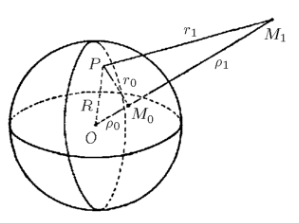
\includegraphics[width=0.4\linewidth]{img/sphere_green}
	\caption{}
\end{figure}

Точки $M_0$ и $M_1$ называются сопряженными друг другу. 

Докажем, что для всех точек $P$ на сфере, расстояния до $M_0$ и $M_1$ пропорциональны. Рассмотрим $\triangle OPM_0$ и $\triangle OMP_1$. Они подобны по общему углу и двум пропорциональным сторонам
\begin{equation*}
	\frac{\rho_0}{R} = \frac{R}{\rho_1}, \text{ или } \frac{\abs{OM_0}}{R} = \frac{R}{\abs{OM_1}}.
\end{equation*}
Из подобия следует
\begin{equation} \label{prop}
	\frac{r_0}{r_1} = \frac{\rho_0}{R} = \frac{R}{\rho_1},
\end{equation}
где $r_0 = \abs{\overrightarrow{M_0P}}$, $r_1 = \abs{\overrightarrow{M_1 P}}$. Из пропорции \eqref{prop} получаем  
\begin{equation*}
	r_0 = \frac{\rho_0}{R} r_1
\end{equation*}
для всех точек сферы. Поэтому гармоническая функция $v = -R/\rho_0 \cdot 1/r_1$ на сфере принимает то же значение, что и функция $-1/r_0$. она представляет, очевидно потенциал заряда величины $-R/\rho_0$, помещенного в точку $M_1$.

Таким образом 
\begin{equation} \label{final_green}
	G(P, M_0) = \frac{1}{4 \pi} \Bigg(\frac{1}{r_0} - \frac{R}{\rho_0} \frac{1}{r_1}\Bigg)
\end{equation}

\paragraph{Функция источника для круга.}\footnote{Т.-С. стр. 346}

Функция источника для круга может быть получена таким же способом, как и функция источника для сферы. В этом случа ее следует искать в виде
\begin{equation}
	G = \frac{1}{2 \pi} \ln{\frac{1}{r}} + v.
\end{equation}

Повторяя рассуждения от \eqref{section} до \eqref{final_green}, мы найдем функцию $G$ в виде 
\begin{equation}
	G = \frac{1}{2 \pi} \Bigg[\ln{\frac{1}{r_0}} - \ln{\frac{R}{\rho_0} \frac{1}{r_1}}\Bigg],
\end{equation}
где $\rho_0 = \abs{OM_0}$, $r_0 = \abs{M_0 P}$, $r_1 = \abs{M_1 P}$, $R = \abs{OP}$ --- радиус круга (см. рис. \ref{circle_green}).
\begin{figure}[H]
	\centering
	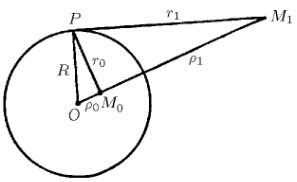
\includegraphics[width=0.4\linewidth]{img/circle_green}
	\caption{}
	\label{circle_green}
\end{figure}
Нетрудно убедиться в том, что определенная таким образом гармоническая функция обращается в нуль на границе: $G|_{C} = 0$.

\paragraph{Функция источника для полупространства.}\footnote{Т.-С. стр. 347}

Найдем функцию источника для полупространства $z > 0$. Поместим в точку $M_0(x_0, y_0, x_0)$ единичный заряд, который создает в неограниченном пространстве поле, потенциал которого определяется функцией 
\begin{equation*}
	\frac{1}{4 \pi} \frac{1}{R_{M_0 M}}, \text{ где } R_{M_0 M} = \sqrt{(x - x_0)^2 + (y - y_0)^2 + (z - z_0)^2}.
\end{equation*}
Нетрудно видеть, что "индуцированное поле" $v$ является полем отрицательного единичного заряда, помещенного в точку $M_1(x_0, y_0, -z_0)$, являющуюся зеркальным изображением точки $M_0$ в плоскости $z = 0$ (рис. \ref{halfdim_green}). 
Функция $G$, равная
\begin{equation*}
	G(M, M_0) = \frac{1}{4 \pi R_0} - \frac{1}{4 \pi R_1},
\end{equation*}
где
\begin{align*}
	R_0 = \abs{\overrightarrow{M_0 M}} = \sqrt{(x - x_0)^2 + (y - y_0)^2 + (z - z_0)^2}, \\
	R_1 = \abs{\overrightarrow{M_1 M}} = \sqrt{(x - x_0)^2 + (y - y_0)^2 + (z - z_0)^2}, \\
\end{align*}
обращается в нуль при $z = 0$ и имеет нужную особенность в точке $M_0$.

\begin{figure}[H]
	\centering
	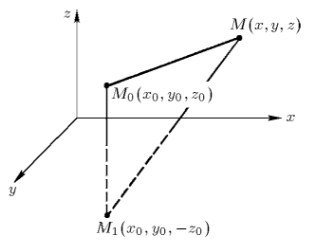
\includegraphics[width=0.4\linewidth]{img/halfdim_green}
	\caption{}
	\label{halfdim_green}
\end{figure}
